\documentclass[11pt,a4paper]{article}

\usepackage[utf8]{inputenc}
\usepackage[T1]{fontenc}
\usepackage{amsmath,amssymb}
\usepackage{booktabs}
\usepackage{caption}
\usepackage{tabularx}
\usepackage{geometry}
\usepackage{graphicx}
\usepackage{hyperref}
\usepackage[round,authoryear]{natbib}
\usepackage{tikz}
\usetikzlibrary{arrows.meta,positioning,shapes.geometric}

\geometry{margin=1in}
\captionsetup[table]{skip=7pt}
\captionsetup[figure]{skip=6pt}
\graphicspath{{../experiments/outputs/}}
\newcolumntype{Y}{>{\raggedright\arraybackslash}X}

\title{Bayesian Decision and Uncertainty:\\Asymmetric Clinical Triage for Skin Lesions}
\author{}
\date{}

\begin{document}

\maketitle

\begin{abstract}

\noindent Automated dermoscopic image analysis is often summarized by symmetric metrics such as accuracy or area under the receiver operating characteristic curve, yet melanoma triage is not a symmetric decision problem. Missing a melanoma is clinically more costly than referring a benign lesion for review. This report studies the binary melanoma-versus-benign task specified for HAM10000 and ISIC 2018 by comparing a classical HSV histogram Gaussian mixture model with an EfficientNet-B0 classifier using Monte Carlo Dropout. The central question is not only which model ranks lesions better, but how calibrated probabilities, asymmetric Bayesian loss, and epistemic uncertainty alter triage behavior. On the lesion-aware held-out test split used here, the Platt-calibrated deep model reaches an AUC of 0.820 compared with 0.805 for the HSV baseline, with a Brier score of 0.080 and test ECE of 0.018. A theoretical 10:1 false-negative to false-positive loss ratio yields 78.5\% sensitivity and 67.1\% specificity, while a calibration-selected 98\% sensitivity operating point reaches 98.0\% test sensitivity at 28.4\% specificity. Adding an MC Dropout triage zone auto-reassures 21.1\% of test lesions with three false negatives among auto-reassured cases. The results support a cautious triage interpretation: probabilities should be calibrated before asymmetric thresholds are applied, and high-uncertainty lesions should be routed to human review rather than treated as ordinary binary predictions.
\end{abstract}

\section{Introduction}

Skin lesion triage is a useful setting for studying Bayesian decision theory because the statistical classification task and the clinical decision task are not identical. A classifier may assign high rank to most melanomas and therefore achieve a strong ROC curve, while still being unsafe at the threshold chosen for deployment. In melanoma screening, the error types are not exchangeable: a false positive can lead to anxiety, specialist review, or biopsy of a benign nevus, but a false negative can delay diagnosis of a potentially lethal malignancy. The assignment therefore asks how a classifier should behave when false negatives are much more costly than false positives, using HAM10000 dermoscopic images and the ISIC 2018 challenge context as the empirical setting.

The motivation for this question is broader than the binary task itself. The ISIC challenges were designed to standardize evaluation in lesion segmentation, attribute detection, and disease classification, and the 2018 challenge emphasized both scale and generalization across acquisition sources \citep{codella2018skin}. HAM10000 was released to address a related bottleneck: public dermoscopy datasets had historically been small, diagnostically narrow, or difficult to access, whereas HAM10000 provides 10,015 images across common pigmented lesion diagnoses \citep{tschandl2018ham10000}. The dataset is nevertheless not a substitute for a prospective clinical trial. It contains repeated images of some lesions, class imbalance, and mixed ground-truth procedures, including histopathology, follow-up, expert consensus, and confocal microscopy \citep{tschandl2018ham10000}. These properties matter because the present task is explicitly about triage, calibration, and uncertainty rather than only image recognition.

This report follows the task specification in three parts. First, a classical generative baseline extracts global HSV colour histograms and fits one Gaussian mixture model per class. This baseline is intentionally limited: it tests how much diagnostic signal is available in global colour distributions alone. Second, a modern discriminative model uses a frozen EfficientNet-B0 backbone with a trained binary classification head, followed by limited fine-tuning of the final feature blocks in the executed experiment. Third, both models are interpreted through Bayesian decision theory. A predicted melanoma probability is not used with a fixed threshold by default; instead, the decision threshold is derived from the false-negative and false-positive loss ratio. Because this rule is only meaningful when probabilities behave as probabilities, the analysis also reports Brier score, expected calibration error, and Monte Carlo Dropout uncertainty.

The contribution of the report is therefore deliberately modest and methodological. It does not claim clinical readiness. It shows how the same held-out test predictions lead to different triage policies when the loss function changes, and why calibration and uncertainty are central to interpreting such policies.

\section{Methods}

The experiment reduces HAM10000 to a binary melanoma triage problem. Melanoma (\texttt{mel}) is the positive class. Melanocytic nevi (\texttt{nv}), benign keratosis-like lesions (\texttt{bkl}), dermatofibroma (\texttt{df}), and vascular lesions (\texttt{vasc}) are treated as benign negatives. Basal cell carcinoma and actinic keratoses are excluded, not because they are unimportant, but because assigning them to the benign class would make the decision rule clinically incoherent: a safe triage system should not be penalized for referring a non-melanoma malignancy or premalignant lesion.

\begin{table}[htbp]
\centering
\caption{Binary task construction after excluding basal cell carcinoma and actinic keratoses.}
\label{tab:dataset}
\begin{tabular}{llrr}
\toprule
Diagnosis & Binary role & Count & Percentage \\
\midrule
\texttt{mel} & melanoma positive & 1,113 & 12.1\% \\
\texttt{nv} & benign negative & 6,705 & 73.1\% \\
\texttt{bkl} & benign negative & 1,099 & 12.0\% \\
\texttt{df} & benign negative & 115 & 1.3\% \\
\texttt{vasc} & benign negative & 142 & 1.5\% \\
\midrule
Total & analyzed images & 9,174 & 100.0\% \\
\bottomrule
\end{tabular}
\end{table}

The split protocol is lesion-aware. HAM10000 includes a \texttt{lesion\_id} field because a single physical lesion may have multiple images. If such images are split independently, visually similar observations of the same lesion can appear in both training and evaluation partitions, inflating performance. The analysis therefore uses grouped splitting so that each \texttt{lesion\_id} belongs to exactly one partition. The executed split contains 4,750 fit images, 1,146 validation images for checkpoint selection, 1,418 calibration images for Platt scaling and threshold selection, and 1,860 held-out test images for final evaluation. The melanoma prevalence is 13.2\% in the fit split, 12.5\% in validation, 10.0\% in calibration, and 10.8\% in test.

The classical pipeline uses colour as a deliberately interpretable baseline. Each image is converted from RGB to HSV, and normalized histograms are extracted for hue, saturation, and value. The resulting vector, denoted by $\phi(x)$, is a compact summary of how colour is distributed in image $x$. It discards where colours occur, but preserves whether the lesion contains darker, redder, or more saturated regions.

For each class, the baseline asks a simple density-estimation question: how likely would this colour histogram be if the lesion were benign, and how likely would it be if the lesion were melanoma? A Gaussian mixture model answers this by representing each class as a weighted sum of $K$ Gaussian components,
\begin{equation}
    p(\phi(x) \mid y=c) = \sum_{k=1}^{K} \pi_{ck}\mathcal{N}\left(\phi(x); \mu_{ck}, \Sigma_{ck}\right),
\end{equation}
where $c \in \{0,1\}$ indicates benign or melanoma, $\pi_{ck}$ is the mixture weight of component $k$, and $\mu_{ck}$ and $\Sigma_{ck}$ describe the mean and covariance of that component. In the implementation, diagonal covariance matrices are used for numerical stability and the number of components is selected by BIC, giving $K=28$ for benign lesions and $K=8$ for melanoma.

The two class likelihoods are then converted into a posterior probability by Bayes' rule. The numerator is the melanoma likelihood multiplied by the melanoma prior; the denominator normalizes this quantity against the corresponding benign likelihood:
\begin{equation}
    p(y=1 \mid x) =
    \frac{p(\phi(x)\mid y=1)p(y=1)}
    {p(\phi(x)\mid y=1)p(y=1)+p(\phi(x)\mid y=0)p(y=0)}.
\end{equation}
\noindent This model can exploit global colour differences, but it cannot represent local border irregularity, asymmetry, streaks, or pigment networks.

The deep pipeline uses EfficientNet-B0 because it provides a compact ImageNet-pretrained convolutional feature extractor \citep{tan2019efficientnet}. Images are resized to $224 \times 224$, normalized with ImageNet statistics, and augmented with flips, modest rotation, and colour jitter during training. The classification head consists of dropout followed by a single logit. The logit $z_i$ is an unconstrained score; applying the sigmoid function $\sigma(z_i)$ maps it to a number between zero and one.

The model is trained with unweighted binary cross-entropy. This loss rewards high probabilities for melanoma images and low probabilities for benign images:
\begin{equation}
    \mathcal{L} = -\frac{1}{N}\sum_{i=1}^{N}
    \left[y_i\log\sigma(z_i)+(1-y_i)\log(1-\sigma(z_i))\right].
\end{equation}
Here $y_i=1$ for melanoma and $y_i=0$ for benign lesions. The unweighted form is deliberate. Class weights can help optimization under imbalance, but they also shift the logit intercept and make $\sigma(z)$ less clean as an estimate of the posterior probability. The executed run therefore applies clinical asymmetry at decision time, after calibration, rather than embedding it simultaneously in the training loss.

Calibration is handled with Platt scaling on the held-out calibration partition. The purpose of this step is not to change the ranking of lesions, but to make the numerical probabilities better match observed frequencies. Platt scaling learns a slope and an intercept on top of the neural-network logit:
\begin{equation}
    \hat{p}(y=1\mid x) = \sigma(az+b).
\end{equation}
\noindent The slope $a$ adjusts the spread of the scores, while the intercept $b$ adjusts the base-rate shift. The intercept is particularly relevant when class imbalance or model bias shifts the predicted prevalence. Calibration quality is summarized with the Brier score,
\begin{equation}
    \mathrm{Brier} = \frac{1}{N}\sum_{i=1}^{N}\left(\hat{p}_i-y_i\right)^2,
\end{equation}
and expected calibration error (ECE). For $M$ probability bins $B_m$, ECE is
\begin{equation}
    \mathrm{ECE} = \sum_{m=1}^{M}\frac{|B_m|}{N}
    \left|\mathrm{acc}(B_m)-\mathrm{conf}(B_m)\right|,
\end{equation}
where $\mathrm{acc}(B_m)$ is the empirical positive frequency and $\mathrm{conf}(B_m)$ is the mean predicted probability in the bin \citep{guo2017calibration}. ECE is easy to read but should be interpreted cautiously because it depends on binning and may hide local miscalibration near clinically important thresholds.

The Bayesian decision rule compares the expected harm of two actions. If the model auto-reassures a lesion as benign, the possible harm is a missed melanoma, weighted by the calibrated melanoma probability $\hat{p}$. If the model refers a lesion, the possible harm is an unnecessary referral or biopsy, weighted by the benign probability $1-\hat{p}$. Thus predicting benign has expected loss $\hat{p}L_{FN}$, and referral has expected loss $(1-\hat{p})L_{FP}$. Referral is preferred when
\begin{equation}
    \hat{p}L_{FN} > (1-\hat{p})L_{FP},
\end{equation}
which yields the threshold
\begin{equation}
    \tau = \frac{L_{FP}}{L_{FP}+L_{FN}}.
\end{equation}
\noindent For a $10:1$ false-negative to false-positive cost ratio, $\tau=1/11 \approx 0.091$. The threshold is low because even a small calibrated probability of melanoma may justify referral when the cost of missing melanoma is high.

Finally, Monte Carlo Dropout is used to estimate epistemic uncertainty. Dropout remains active during inference, so the same image is passed through several slightly different subnetworks. This produces $T=30$ stochastic probabilities $p_t$. Their average, $\bar{p}$, is the final probability used for thresholding. The variation across the $T$ values indicates how stable the model is for that image. Predictive entropy measures total uncertainty,
\begin{equation}
    H[\bar{p}] = -\bar{p}\log\bar{p}-(1-\bar{p})\log(1-\bar{p}),
\end{equation}
while mutual information estimates model disagreement:
\begin{equation}
    MI = H[\bar{p}] - \frac{1}{T}\sum_{t=1}^{T}H[p_t].
\end{equation}

\noindent High mutual information indicates that different dropout subnetworks disagree, a practical signal that the lesion should be treated as uncertain rather than automatically cleared.

\begin{figure}[htbp]
\centering
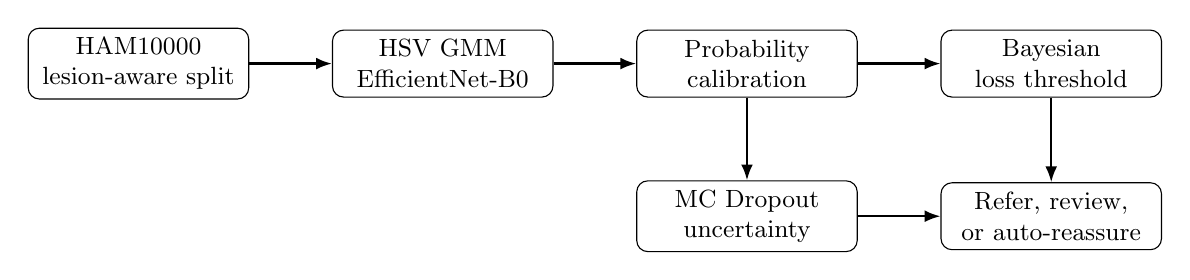
\begin{tikzpicture}[
    node distance=1.05cm,
    box/.style={draw, rounded corners, align=center, minimum width=2.8cm, minimum height=0.85cm, font=\small},
    arrow/.style={-{Latex[length=2mm]}, thick}
]
\node[box] (data) {HAM10000\\lesion-aware split};
\node[box, right=of data] (models) {HSV GMM\\EfficientNet-B0};
\node[box, right=of models] (cal) {Probability\\calibration};
\node[box, right=of cal] (decision) {Bayesian\\loss threshold};
\node[box, below=of cal] (unc) {MC Dropout\\uncertainty};
\node[box, right=of unc] (triage) {Refer, review,\\or auto-reassure};
\draw[arrow] (data) -- (models);
\draw[arrow] (models) -- (cal);
\draw[arrow] (cal) -- (decision);
\draw[arrow] (cal) -- (unc);
\draw[arrow] (decision) -- (triage);
\draw[arrow] (unc) -- (triage);
\end{tikzpicture}
\caption{Evaluation flow for the task. The image classifier estimates melanoma probability, calibration makes the probability usable for decision thresholds, and MC Dropout provides an uncertainty signal for lesions that should not be handled by a binary threshold alone.}
\label{fig:workflow}
\end{figure}


\section{Results}

The classical and deep pipelines first differ in ranking performance. The HSV GMM reaches an AUC of 0.805 on the held-out test split, whereas the EfficientNet-B0 MC Dropout predictive mean reaches an AUC of 0.820 after Platt calibration. The ROC curves in Figure~\ref{fig:roc} show that the deep model ranks lesions modestly better than global colour histograms, although the separation is far from a clinically definitive diagnostic test.

\begin{figure}[htbp]
\centering
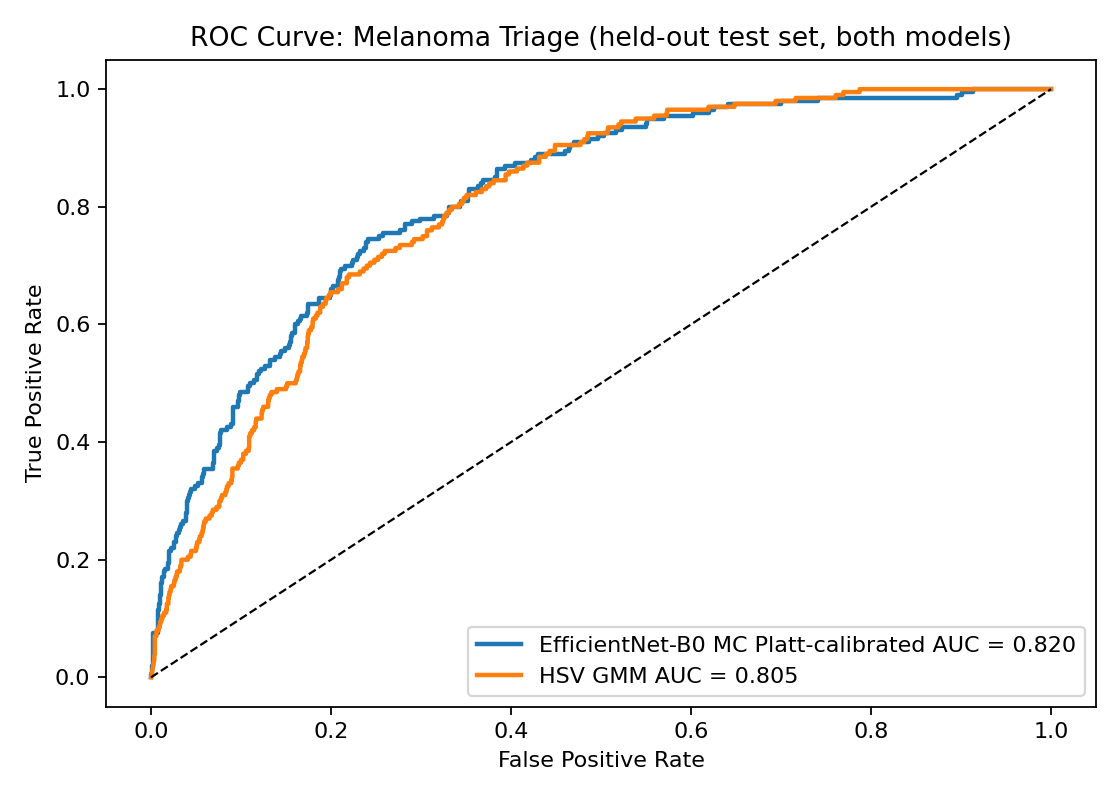
\includegraphics[width=0.86\textwidth]{roc_curve_triage.png}
\caption{Receiver operating characteristic curves for the Platt-calibrated deep model and the HSV GMM baseline on the held-out test split. The deep model has slightly stronger ranking performance, but ROC AUC alone does not specify the triage operating point.}
\label{fig:roc}
\end{figure}

The training trajectory supports the interpretation that the deep model learned useful discriminative structure. Validation AUC improved from 0.705 after the first head-training epoch to 0.853 after fine-tuning. On the held-out test split, the calibrated Brier score was 0.080 and test ECE was 0.018, improved from a raw ECE of 0.067. These values indicate that calibration made the probabilities more usable for decision-theoretic thresholding, although the threshold behavior below shows that ranking and calibration do not remove the referral tradeoff.

\begin{table}[htbp]
\centering
\caption{Model comparison on the held-out test split. The GMM is trained on a fit-split subsample for speed; both models are evaluated on the same test lesions.}
\label{tab:model-comparison}
\begin{tabularx}{\textwidth}{Y Y c Y}
\toprule
Model & Main feature representation & AUC & Calibration notes \\
\midrule
HSV GMM & Global HSV histograms & 0.805 & Generative posterior from coarse global colour features; ECE 0.143 \\
EfficientNet-B0 + MC Dropout & Learned dermoscopic morphology & 0.820 & Platt-calibrated probabilities; Brier 0.080, ECE 0.018 \\
\bottomrule
\end{tabularx}
\end{table}

The calibration summary in Figure~\ref{fig:calibration} explains why the decision analysis cannot rely on AUC alone. The reliability diagram compares predicted melanoma probability with empirical melanoma frequency on the held-out test split. Calibration is important operationally: the theoretical $10:1$ threshold refers 37.8\% of test lesions rather than collapsing into universal referral, but it still leaves a substantial number of missed melanomas.

\begin{figure}[htbp]
\centering
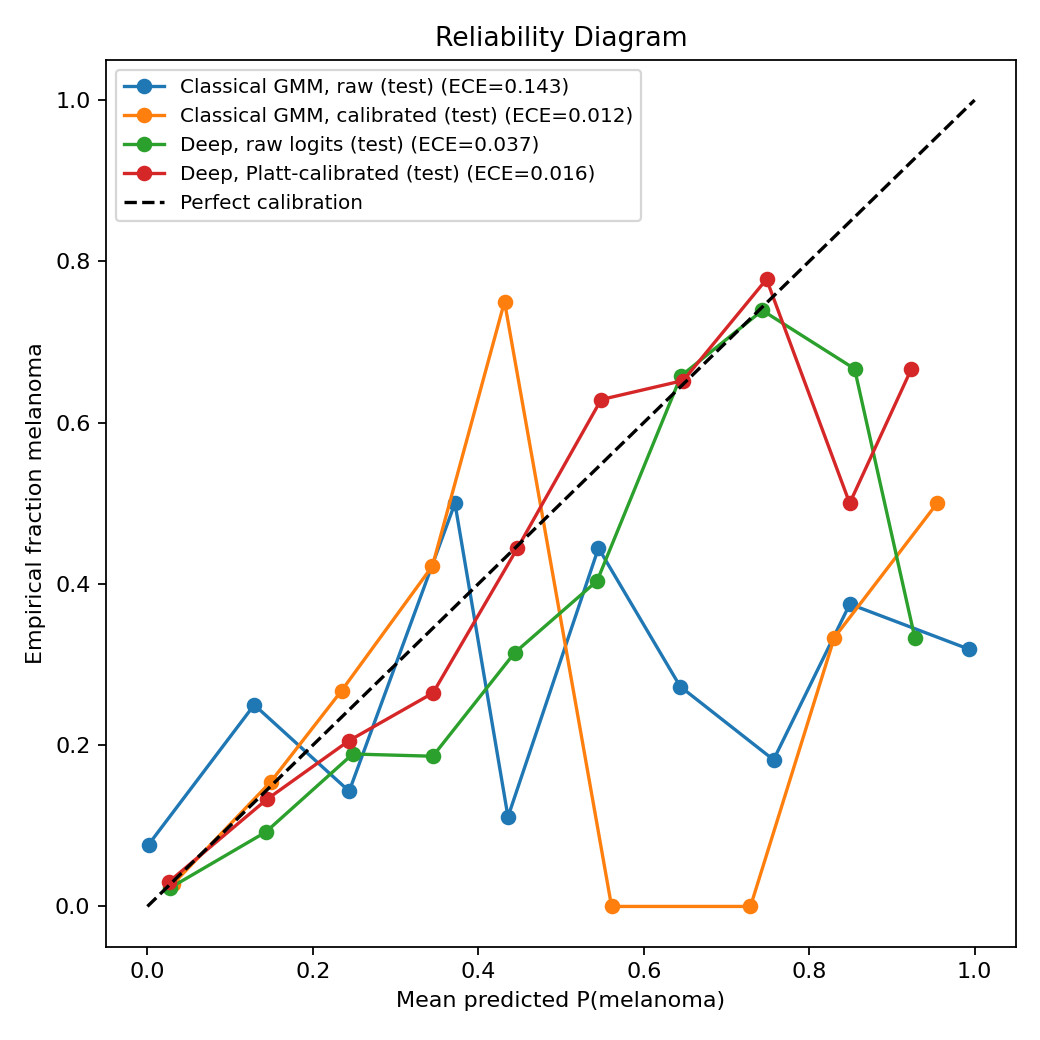
\includegraphics[width=0.9\textwidth]{reliability_diagram.png}
\caption{Reliability diagram generated from the held-out test predictions. Calibration quality determines whether a nominal Bayesian threshold can be interpreted as a probability threshold.}
\label{fig:calibration}
\end{figure}

The central effect of asymmetric loss is visible in Table~\ref{tab:thresholds}. At the symmetric threshold of 0.5, specificity is high but sensitivity is only 15.5\%, which is clinically unacceptable for melanoma screening. Lowering the threshold according to a $10:1$ loss ratio raises sensitivity to 78.5\% and keeps specificity at 67.1\%, referring 37.8\% of test lesions. A still more conservative $20:1$ threshold raises sensitivity to 89.0\% at the cost of a 50.0\% referral rate. The theoretical $10:1$ threshold therefore gives a manageable referral burden, but it still misses 43 melanomas in this held-out test split.

\begin{table}[htbp]
\centering
\caption{Held-out test triage metrics under theoretical Bayesian thresholds from asymmetric loss. Thresholds are applied to Platt-calibrated MC Dropout predictive means.}
\label{tab:thresholds}
\begin{tabular}{lrrrrrr}
\toprule
Cost ratio & Threshold & Sensitivity & Specificity & Precision & Referral & FN \\
\midrule
1:1  & 0.500 & 0.155 & 0.989 & 0.633 & 0.026 & 169 \\
5:1  & 0.167 & 0.645 & 0.808 & 0.289 & 0.240 & 71 \\
10:1 & 0.091 & 0.785 & 0.671 & 0.223 & 0.378 & 43 \\
20:1 & 0.048 & 0.890 & 0.547 & 0.191 & 0.500 & 22 \\
\bottomrule
\end{tabular}
\end{table}

Because a theoretical loss ratio does not automatically guarantee a target clinical sensitivity on finite data, the analysis also selects thresholds on the calibration split by requiring minimum sensitivity and then evaluates them once on the held-out test split. Table~\ref{tab:operating-points} shows that a calibration-selected threshold for at least 98\% sensitivity gives 98.0\% test sensitivity, 28.4\% specificity, and four false negatives. Requiring at least 99\% calibration sensitivity does not guarantee 99\% sensitivity on test; it reaches 98.5\% sensitivity with three false negatives while referring 78.9\% of lesions. These operating points are more clinically interpretable than a single cost ratio because they state the intended safety level directly and expose how much referral burden is needed.

\begin{table}[htbp]
\centering
\caption{Sensitivity-constrained thresholds selected on the calibration split and evaluated on the held-out test split. Each row chooses the highest-specificity calibration threshold satisfying the target sensitivity.}
\label{tab:operating-points}
\begin{tabular}{lrrrrr}
\toprule
Target sensitivity & Threshold & Test sensitivity & Specificity & Referral & FN \\
\midrule
0.95 & 0.018 & 0.975 & 0.357 & 0.679 & 5 \\
0.98 & 0.012 & 0.980 & 0.284 & 0.745 & 4 \\
0.99 & 0.009 & 0.985 & 0.235 & 0.789 & 3 \\
\bottomrule
\end{tabular}
\end{table}

Figure~\ref{fig:uncertainty} shows why a single threshold is still an incomplete triage rule. Mutual information increases in the ambiguous middle of the probability range, and the highest-uncertainty cases include melanoma examples that are not extreme high-probability predictions. A clinically cautious workflow should therefore avoid interpreting all below-threshold cases as equally safe.

\begin{figure}[htbp]
\centering
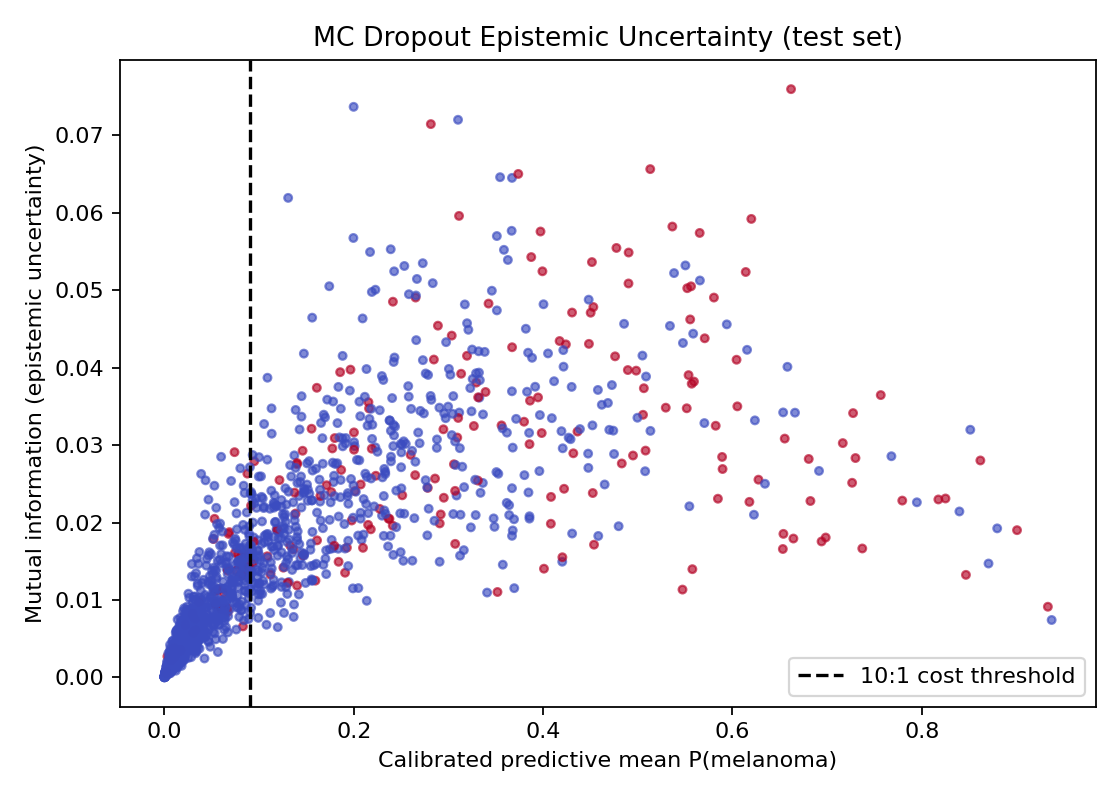
\includegraphics[width=0.86\textwidth]{uncertainty_scatter.png}
\caption{MC Dropout mutual information versus predicted melanoma probability. The dashed vertical line marks the $10:1$ Bayesian threshold. Points with high mutual information indicate model disagreement and are better interpreted as manual-review cases than as ordinary confident predictions.}
\label{fig:uncertainty}
\end{figure}

\section{Discussion and Conclusion}

The experiment illustrates the distinction between discrimination, calibration, and decision-making. The deep model discriminates only modestly better than the HSV GMM on this run, even though it can use spatial morphology that a global colour histogram discards. Better AUC still does not by itself solve the clinical problem. The Bayesian rule asks a different question: given a calibrated probability and an explicit loss matrix, which action minimizes expected harm? With unweighted training and Platt calibration, the predicted probabilities become more usable for this decision rule: ECE is 0.018, and the $10:1$ threshold produces a referral rate of 37.8\% rather than collapsing into universal referral.

The calibrated $10:1$ operating point is therefore informative but not sufficient. It refers 37.8\% of lesions and reaches only 78.5\% sensitivity, which is too low for a screening-oriented melanoma triage system. The sensitivity-constrained thresholds give a clearer safety interpretation. If the system must maintain approximately 98\% sensitivity, the test referral rate rises to 74.5\%; if the calibration target is raised to 99\%, the test referral rate rises to 78.9\% while test sensitivity reaches 98.5\%. These values are operationally expensive, but they make the tradeoff explicit rather than hiding it behind accuracy or AUC.

The uncertainty analysis suggests a practical compromise: triage should not be forced into a single binary action. A more clinically plausible policy has three zones. Lesions with low calibrated melanoma probability and low epistemic uncertainty can be auto-reassured. Lesions with high probability should be referred urgently. Lesions in between, or lesions with high MC Dropout mutual information, should be sent to manual review. In the held-out test run, this policy auto-reassures 21.1\% of lesions with three false negatives among auto-reassured cases, while urgent referrals are much more enriched for melanoma than the broad low-threshold referral sets. This framing fits the assignment's uncertainty requirement more naturally than using MC Dropout only as a plot, because it gives uncertainty a decision role.

The uncertainty-aware triage zone makes this practical. Using the calibration-selected 99\% sensitivity threshold as the low-risk cutoff and the 95th percentile calibration mutual information as an uncertainty cutoff, the model auto-reassures 393 test lesions (21.1\%), sends 1,418 lesions (76.2\%) to manual review, and marks 49 lesions (2.6\%) as urgent referrals. There are three melanomas among the auto-reassured cases, corresponding to 98.5\% sensitivity after auto-reassurance, and the urgent-referral group has 63.3\% precision. This is a conservative workflow, but it gives MC Dropout a direct decision role.

\begin{table}[htbp]
\centering
\caption{Three-zone triage policy using calibrated probability and MC Dropout mutual information. Low-risk auto-reassurance requires both low predicted melanoma probability and low epistemic uncertainty.}
\label{tab:triage-zone}
\begin{tabular}{lrr}
\toprule
Triage zone metric & Value & Count \\
\midrule
Auto-reassured lesions & 21.1\% & 393 \\
Manual-review lesions & 76.2\% & 1,418 \\
Urgent-referral lesions & 2.6\% & 49 \\
False negatives among auto-reassured & -- & 3 \\
Sensitivity after auto-reassurance & 98.5\% & -- \\
Urgent-referral precision & 63.3\% & -- \\
\bottomrule
\end{tabular}
\end{table}


Several limitations remain. HAM10000 is a valuable benchmark, but it is retrospective, multi-source, and partly labeled through non-histopathological procedures \citep{tschandl2018ham10000}. The ISIC challenge literature also emphasizes that algorithms with similar benchmark scores can differ in their ability to generalize to external data \citep{codella2018skin}. The present experiment uses one lesion-aware split rather than repeated external validation, and the GMM baseline is deliberately simple. The calibration split is internal to the same HAM10000 training pool rather than drawn from an external cohort. The findings should therefore be interpreted as a controlled demonstration of Bayesian triage behavior rather than evidence for deployment.

In summary, asymmetric melanoma triage cannot be reduced to maximizing accuracy. A classifier must rank lesions, produce calibrated probabilities, and expose uncertainty. Bayesian decision theory then makes the clinical tradeoff explicit: lowering the threshold can reduce false negatives, but the referral burden depends strongly on calibration and class separation. The safest interpretation of this experiment is therefore not that the model should autonomously diagnose melanoma, but that calibrated probability and MC Dropout uncertainty can structure a conservative referral, review, and auto-reassurance workflow.

\newpage
\appendix
\section{Supporting Material}

Figure~\ref{fig:training} shows the training trajectory that supports the reported deep-model result. The curve is placed in the appendix to keep the main Results section focused on evaluation behavior rather than training diagnostics.

\begin{figure}[htbp]
\centering
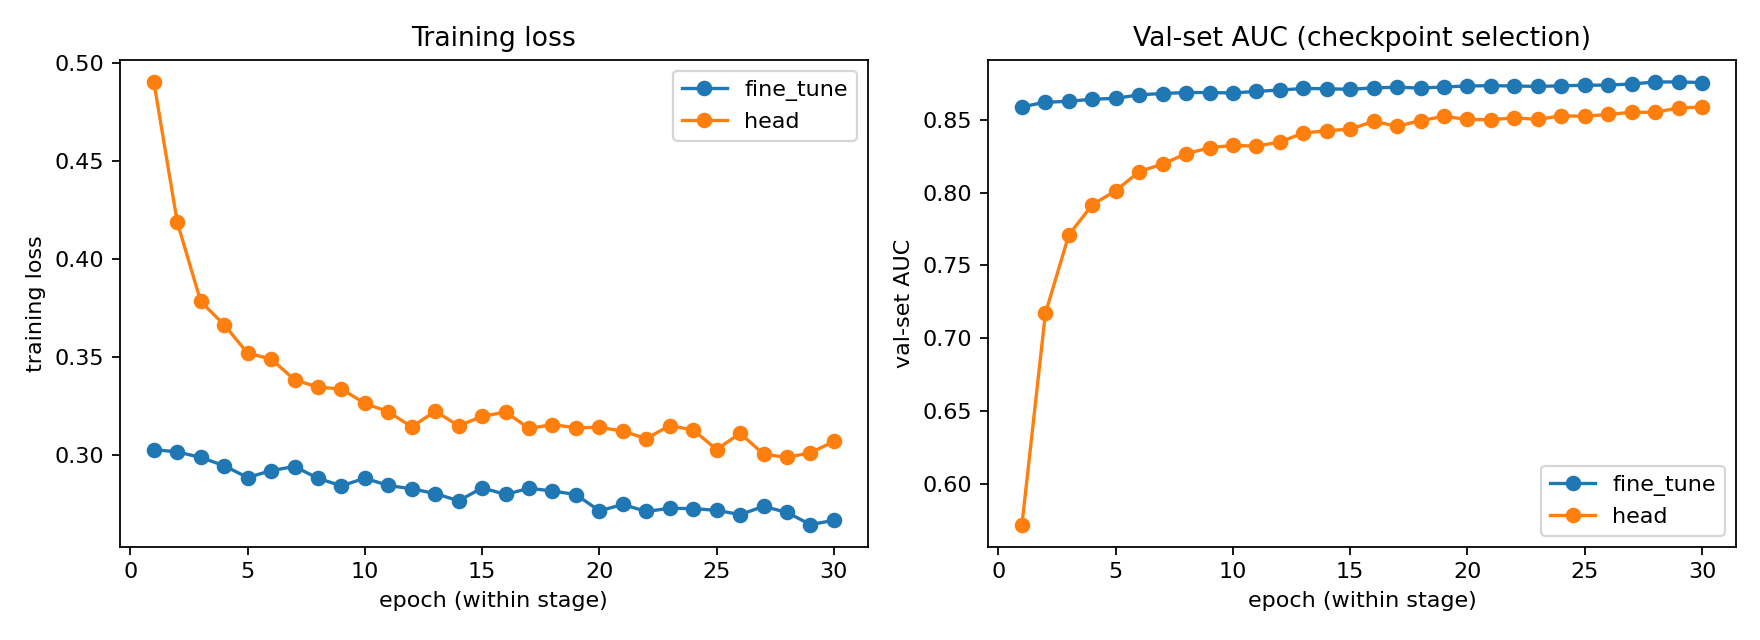
\includegraphics[width=0.82\textwidth]{training_curves.png}
\caption{Training loss and validation AUC over the head-training and fine-tuning stages. Discriminative performance improves before plateauing near validation AUC 0.853.}
\label{fig:training}
\end{figure}

\begin{figure}[htbp]
\centering
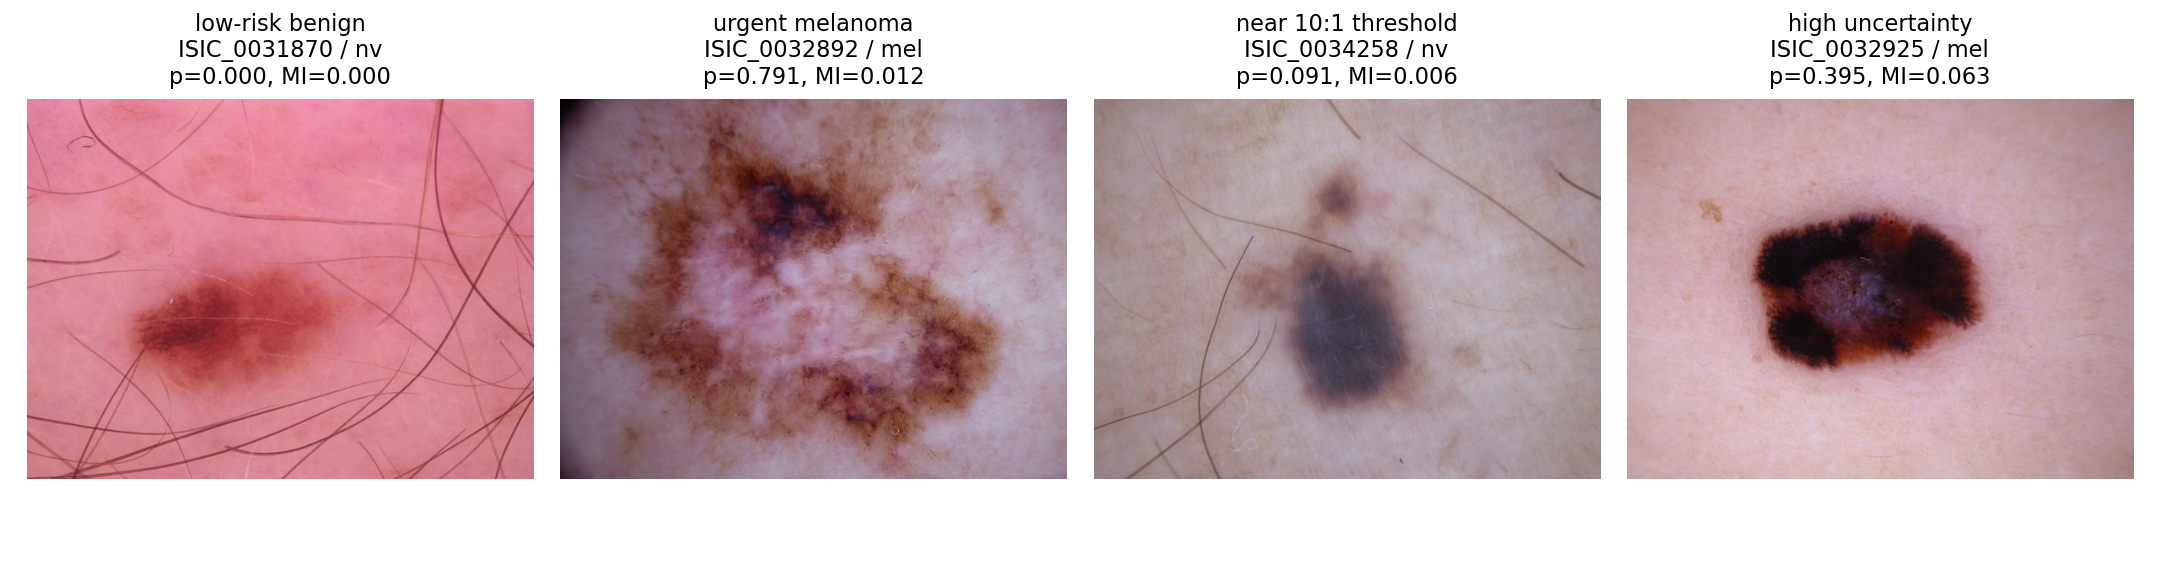
\includegraphics[width=0.98\textwidth]{example_lesions_grid.png}
\caption{Example held-out test lesions from HAM10000. The four panels pair the dermoscopic image with the model role, image identifier, diagnostic label, predicted melanoma probability, and MC Dropout mutual information.}
\label{fig:example-lesions}
\end{figure}

Representative test examples make the same point at the individual-observation level. Table~\ref{tab:examples} includes a very low-probability benign nevus, a high-probability melanoma, a case close to the $10:1$ threshold, and high-uncertainty manual-review examples. These examples are not selected as clinical case studies, since the local repository does not include the image pixels; they are included to make the numerical behavior of the triage rule concrete.

\begin{table}[htbp]
\centering
\caption{Example test predictions from the held-out test run. The $10:1$ threshold is 0.091, while the low-risk triage threshold selected for at least 99\% calibration sensitivity is 0.009.}
\label{tab:examples}
\begin{tabular}{lllrr}
\toprule
Image ID & Diagnosis & Role & $p(\mathrm{mel})$ & Mutual information \\
\midrule
ISIC\_0027841 & \texttt{nv} & low-risk benign & 0.0001 & 0.0000 \\
ISIC\_0032970 & \texttt{mel} & urgent melanoma & 0.8296 & 0.0131 \\
ISIC\_0034118 & \texttt{mel} & near $10:1$ threshold & 0.0907 & 0.0113 \\
ISIC\_0032547 & \texttt{mel} & high uncertainty & 0.4382 & 0.0409 \\
ISIC\_0033437 & \texttt{bkl} & high uncertainty & 0.4925 & 0.0480 \\
\bottomrule
\end{tabular}
\end{table}


\newpage
\bibliographystyle{plainnat}
\bibliography{skin_lesion_triage_refs}

\end{document}
